\documentclass[UTF8]{ctexart}

\usepackage{subfiles}  

%下面的语句, 引入你的头部设置文件
\usepackage{C:/phpStorm_proj/02_myself_ID_EGO/+100_latex_all_math_sel/myPreamble} 
%必须是绝对路径,才能让各个tex在单独编译时使用到

\title{积分}


%---------------------------------


\begin{document}
	\tableofcontents % 生成目录
	\date{} % 若不写这句, 则默认也会渲染出日期, 所以我们要手动赋空值
	\maketitle  %这行代码, 让你前面的 title, author, date生效
	
	\part{积分 integral}
	
	对于曲线f 下的面积, 如果我们能找到一个函数I 来表示它, 那么这个函数I, 就叫做f的``积分".
	
	积分很有用, 是因为很多生活中实际的问题, 都能近似成``大量很小的东西加起来". 而这样的问题都能转化成求某图像下的面积. 所以, 我们要找的, 就是这个能表示面积的"积分函数".
	
	
	
	
	
	
	\part{不定积分 indefinite integral : 即``原函数"}
	
	一个原函数, 求其导数, 能得到"导函数". \textbf{反过来, 从``导函数"算出其``原函数"的过程, 就是求其``不定积分". 换言之, ``原函数"的别名就是"不定积分".}
	
	如: ``原函数"是 F(x), 其``导函数"是 D(x), 即: $ F'(x) = D(x)$, 则  原函数 F(x) 就是 D(x) 的其中一个原函数. \\
	
	为什么是``其中一个"原函数? 因为可以有无穷多个原函数, 它们都能得到同一个导函数. 比如, 这些原函数: $x^2,  x^2+3$, 它们都能得到同一个导函数 $2x$.
	
	其规律就是: $\left( \underset{\text{原函数}}{\underbrace{F\left( x \right) }}+\underset{\text{常数}}{\underbrace{C}} \right) '=\underset{\text{导函数}}{\underbrace{D\left( x \right) }} $ \\
	\\
	
	
\includegraphics[width=0.3\textwidth]{/0055.png} \\
	
	所以, 从``导函数"来反求其``原函数", 就是求``不定积分". 因此, ``原函数"的别名就是``不定积分".
	
	即: $\int_{}^{}{\underset{\text{导函数}}{\underbrace{D\left( x \right) }}dx=\underset{\text{原函数}}{\underbrace{F\left( x \right) }}+\underset{\text{常数}}{\underbrace{C}}} $ \\
	
	我们也就有:
	$	\dfrac{d}{dx}\left[ \underset{\text{原函数}}{\underbrace{\int_{}^{}{\underset{\text{导函数}}{\underbrace{f\left( x \right) }}dx}}} \right] =\underset{\text{导函数}}{\underbrace{f\left( x \right) }}	$ ← 相当于 先ctrl+z (恢复到原函数), 再 ctrl+y (重做下一步的求导操作)
	
	也可写作:	
	$	d\left[ \underset{\text{原函数}}{\underbrace{\int_{}^{}{\underset{\text{导函数}}{\underbrace{f\left( x \right) }}dx}}} \right] =\underset{\text{导函数}}{\underbrace{f\text{(}x\text{)}}}dx	$
	
	
	
	
	符号 $\int$ 是英文 sum 的 首字母s 变形. \\
	
	
	
	Σ 和 $\int$ 的区别: 
	
	\begin{tabular}{|l| l| }
		\hline
		Σ &  通常是对``有限个", 或者``离散的量"求和。 \\
		\hline
		$\int$ & 是对``无穷个"连续的``无穷小量"的求和 \\
		\hline
	\end{tabular} \\

	类似的:
	
	\begin{tabular}{|l| l| }
		\hline
		Δ & 表示``有限小"的变量. \\
		\hline
		dx & 表示``无穷小"变量. 有 x →0 这个``极限"的概念在里面. \\
		\hline
	\end{tabular}





	
	\section{不定积分公式}
	
	\subsection{$\int (0) dx = C$}
	
	
	\subsection{$\int (k) dx = kx + C$}
	
		
	\subsection{$\int (x^n) dx=\frac{1} {n+1} x^{n+1} + C, \quad n \ne -1$}	
	
		
		
	\subsection{$\int (\frac{1} {x}) dx = ln |x| + C$}	
		
		
	\subsection{$\int x dx = \frac{1} {2} x^2 + C$}
		
	\subsection{$\int (e^x) dx = e^x + C$}		

	
	\subsection{$\int (a^x) dx = \frac{a^x} {\ln a} + C$}	
	
		
	\subsection{$ \int (\frac{1} {1+ x^2}) dx = \arctan x + C,  或= -\operatorname{arccot} x + C$}		
	
	\subsection{ $\int (\frac{1} {\sqrt{1-x^2}}) dx = \arcsin x + C,  或= -\arccos x + C$}
	
	\subsection{$ \int \frac{1} {x^2 + a^2} dx = \frac{1} {a} \cdot arctan \frac{x} {a} + C$}
	
	
	\subsection{$\int \frac{1} {x^2 - a^2} dx = \frac{1} {2a} \cdot ln |\frac{x-a} {x+a} | + C$}
		
	\subsection{$\int \frac{1} {\sqrt{x^2 + a^2}} dx = ln | x + \sqrt{x^2 + a^2}|+C$}
	
		\begin{myEnvSample}
			\begin{align*}
					\int_{}^{}{\frac{1}{\sqrt[]{4x^2+9}}dx=\int_{}^{}{\frac{1}{\sqrt[]{4x^2+3^2}}dx}=\frac{1}{2}}\int_{}^{}{\frac{1}{\sqrt[]{\left( 2x \right) ^2+3^2}}d\left( 2x \right) =\frac{1}{2}\ln \left| x+\sqrt[]{\left( 2x \right) ^2+3^2} \right|}+C		
			\end{align*}
		\end{myEnvSample}
	
	
	
	
	\subsection{$\int \frac{1} {\sqrt{x^2 - a^2}}dx  =\ln | x+\sqrt{x^2-a^2}|+C$}
	
	
	\subsection{$\int \frac{1} {\sqrt{a^2 - x^2}}dx = arcsin \frac{x} {a}  +C$}
	
	\subsection{$\int (\sin x) dx = - \cos x + C$}
	
	
	\subsection{$ \int (\cos x) dx = \sin x + C$}
	
	\subsection{$\int (\tan x) dx = -\ln |cos x| + C$}
	
	\subsection{$ \int (\cot x) dx = \ln |sin x| + C$}
	
	\subsection{$\int (\sec x) dx = \ln |sec x + tan x| + C$}
	
	\subsection{$\int (\csc x) dx = \ln |csc x - cot x| + C$}
	
	\subsection{$\int (\ln x) dx = x \ln x - x + C$}
	
	\subsection{$ \int (\sec^2 x) dx = \tan x + C$}
	
	\subsection{$\int (\csc^2 x) dx = - \cot x + C$}
	
	\subsection{$ \int (\sec x \tan x) dx = \sec x + C$}
	

	
	\subsection{$\int (\csc x \cot x) dx = -\csc x + C$}
	




	
	\section{不定积分的性质}
	
	\subsection{$\int [ f(x) \pm g(x) ] dx = \int f(x) dx \pm \int g(x) dx$}
	
	
	\begin{myEnvSample}
		\begin{align*}
	&\int_{}^{}{\frac{\left( x-1 \right) ^3}{x^2}}dx=\int_{}^{}{\frac{x^3-3x^2+3x-1}{x^2}dx}=\int_{}^{}{\left( \text{x}-3+3\frac{1}{\text{x}}-\frac{1}{\text{x}^2} \right)}dx\\
&=\underset{\frac{1}{2}x^2}{\underbrace{\int_{}^{}{\left( \text{x} \right)}dx}}-\underset{3x}{\underbrace{\int_{}^{}{\left( 3 \right)}dx}}+3\underset{\ln\text{|}x|}{\underbrace{\int_{}^{}{\left( \frac{1}{\text{x}} \right)}dx}}-\underset{=\int_{}^{}{\left( x^{-2} \right)}dx=\frac{1}{-2+1}x^{-2+1}}{\underbrace{\int_{}^{}{\left( \frac{1}{\text{x}^2} \right)}dx}}\\
&=\frac{1}{2}x^2-3x+3\ln\text{|}x|+x^{-1}+C
		\end{align*}
	\end{myEnvSample}
	
	
	
	\subsection{$\int (k f(x)) dx = k \cdot \int f(x) dx$}
	
	其中 k 是常数, 且 $ k \ne 0$. 注意: 如果k是一个变量, 如果该变量与x是无关的 (即与``积分变量"无关的), 则可以朝外挪出去; 但如果该变量是与x相关的, 则就不能朝外挪.
	
	
	
	~\\
	\hrule
	~\\
	
	
	\part{求不定积分的方法}
	
	
	
	\section{凑微分法}
	
	求微分, 可以写成(变换成)下面三种形式:	
	 
	 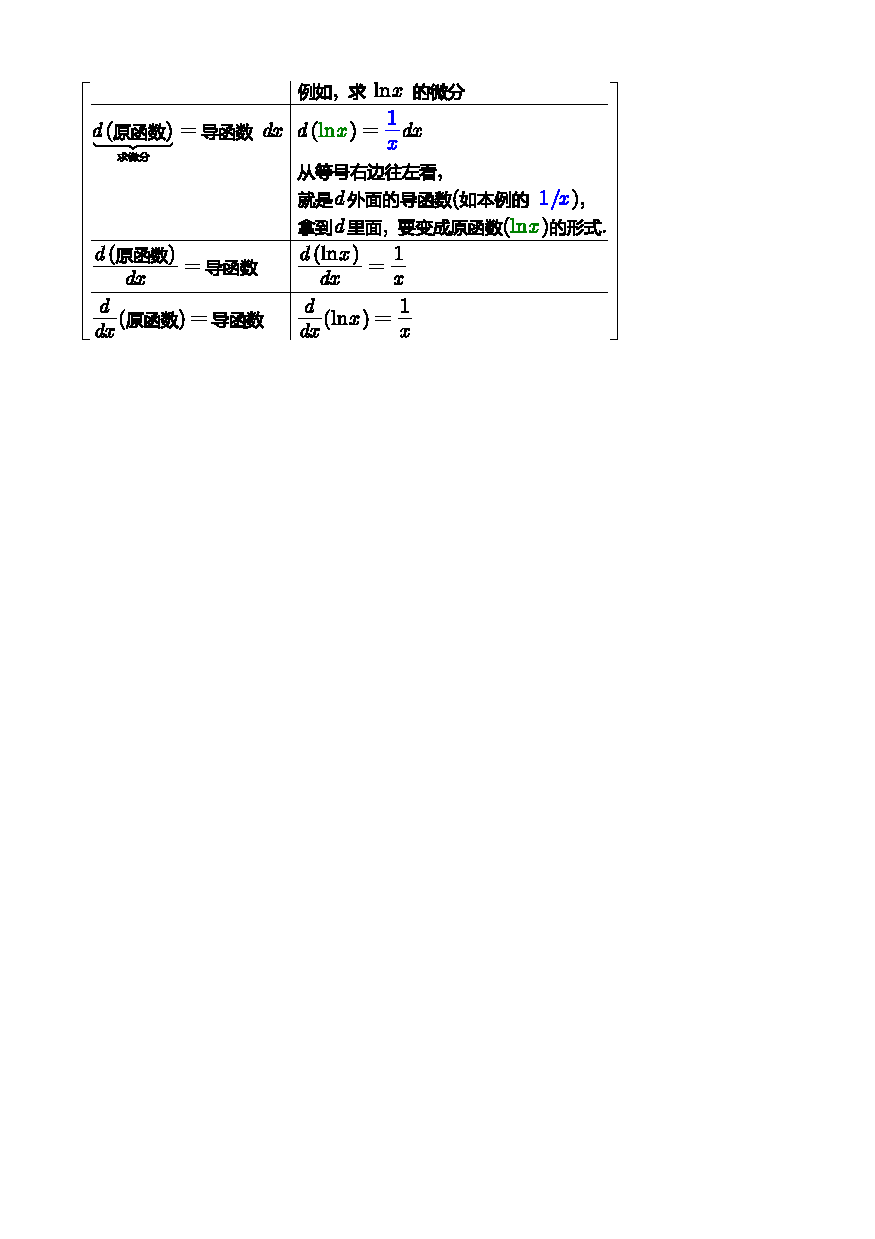
\includegraphics[width=0.7\textwidth]{/0058.pdf}
	 
	
	
	
	
	\section{分部积分法 : $\rightarrow \int_{}^{}{\text{前\ }d\text{(后)}}=\text{前}\cdot \text{后}-\int_{}^{}{\text{后}}\ d\text{(前)}$}
	
	分部积分法 Integration by parts
	
	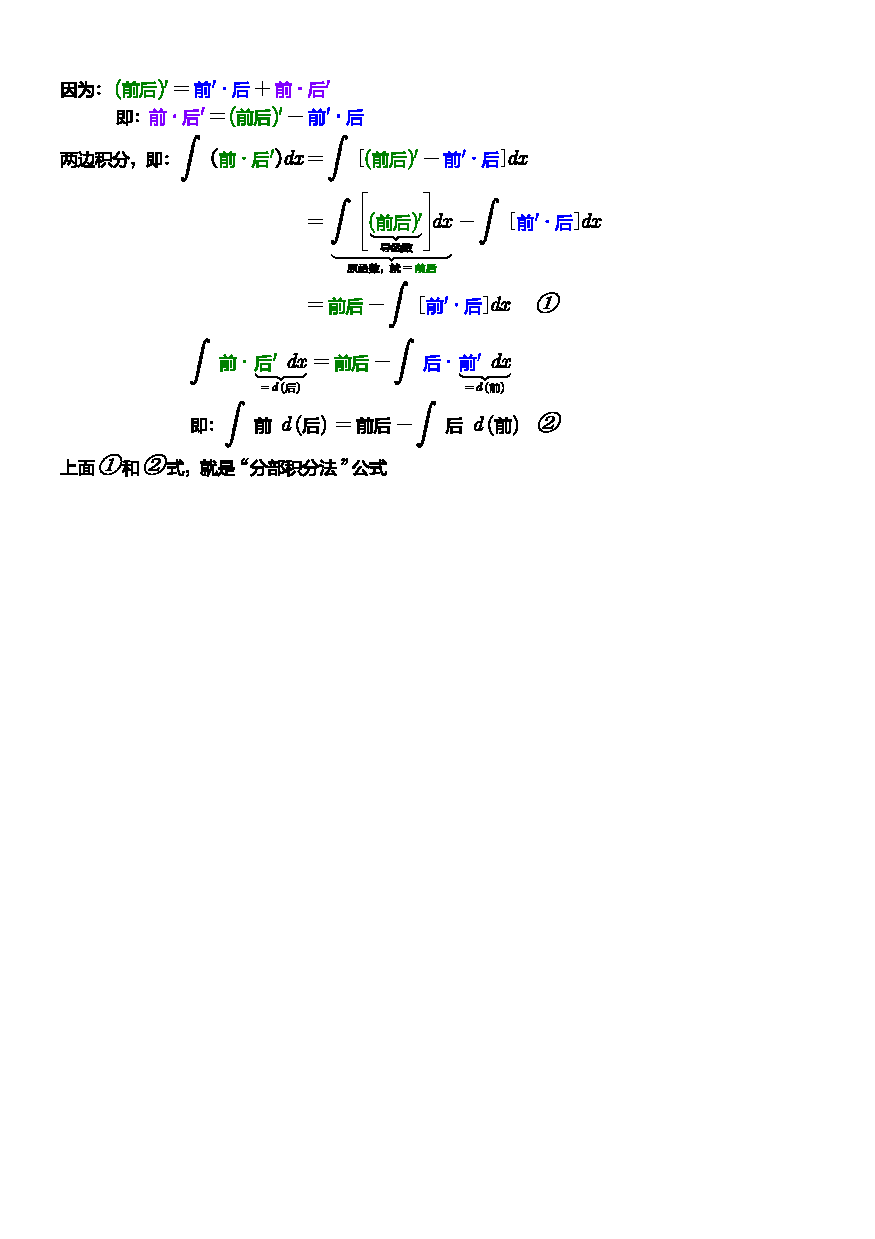
\includegraphics[width=0.7\textwidth]{/0056.pdf} \\
	
	即, 分部积分公式是:	
	\begin{align*}  % 支持每行编号. 若不需要编号, 就用 align*环境		
		&\rightarrow \int_{}^{}{\left( \text{前}\cdot \text{后'} \right) dx}=\text{前}\cdot \text{后}-\int_{}^{}{\left[ \text{前'}\cdot \text{后} \right]}dx\\
		&\rightarrow \int_{}^{}{\text{前\ }d\text{(后)}}=\text{前}\cdot \text{后}-\int_{}^{}{\text{后}}\ d\text{(前)} 
\end{align*}
	
	别忘了关系是: $ \boxed{\int_{}^{}{\text{导函数的世界}}\ d\text{(原函数的世界)}}$ \\
	
	分部积分法的目的, 将是将``不易直接求结果的积分形式",转化为等价的``容易求出结果的积分形式". \\
	
	
	\textbf{``分部积分"的要点是: 谁做``前", 谁做``后"? 即: (1) 谁放d的后面?  (2) 往d里面拿时, 哪个的优先级最高?}
	
	把前面的什么东西, 朝d里面拿? 优先顺序是: $e^x  > \sin x > \cos x > x^n$ \\
	
	\begin{myEnvSample}
		\begin{align*}
	&\int_{}^{}{x\underset{\text{先做}}{\underbrace{e^x\ dx}}}=\int_{}^{}{\underset{\text{前}}{\underbrace{x}}}\ d\underset{\text{后}}{\underbrace{\text{(}e^x\text{)}}}\ \ \gets \text{一前一后两个函数,\ 就用分部积分法}\\
&\int_{}^{}{\text{前\ }d\text{(后)}}=\text{前}\cdot \text{后}-\int_{}^{}{\text{后}}\ d\text{(前)}\\
&\text{本例就是:\ }\int_{}^{}{\underset{\text{前}}{\underbrace{x}}}\ d\underset{\text{后}}{\underbrace{\text{(}e^x\text{)}}}=\underset{\text{前}}{\underbrace{x}}\cdot \underset{\text{后}}{\underbrace{e^x}}-\int_{}^{}{\underset{\text{后}}{\underbrace{e^x}}\ d\text{(}\underset{\text{前}}{\underbrace{x}}\text{)}}=xe^x-e^x+C\\
		\end{align*}
	\end{myEnvSample}
	
	
	\begin{myEnvSample}
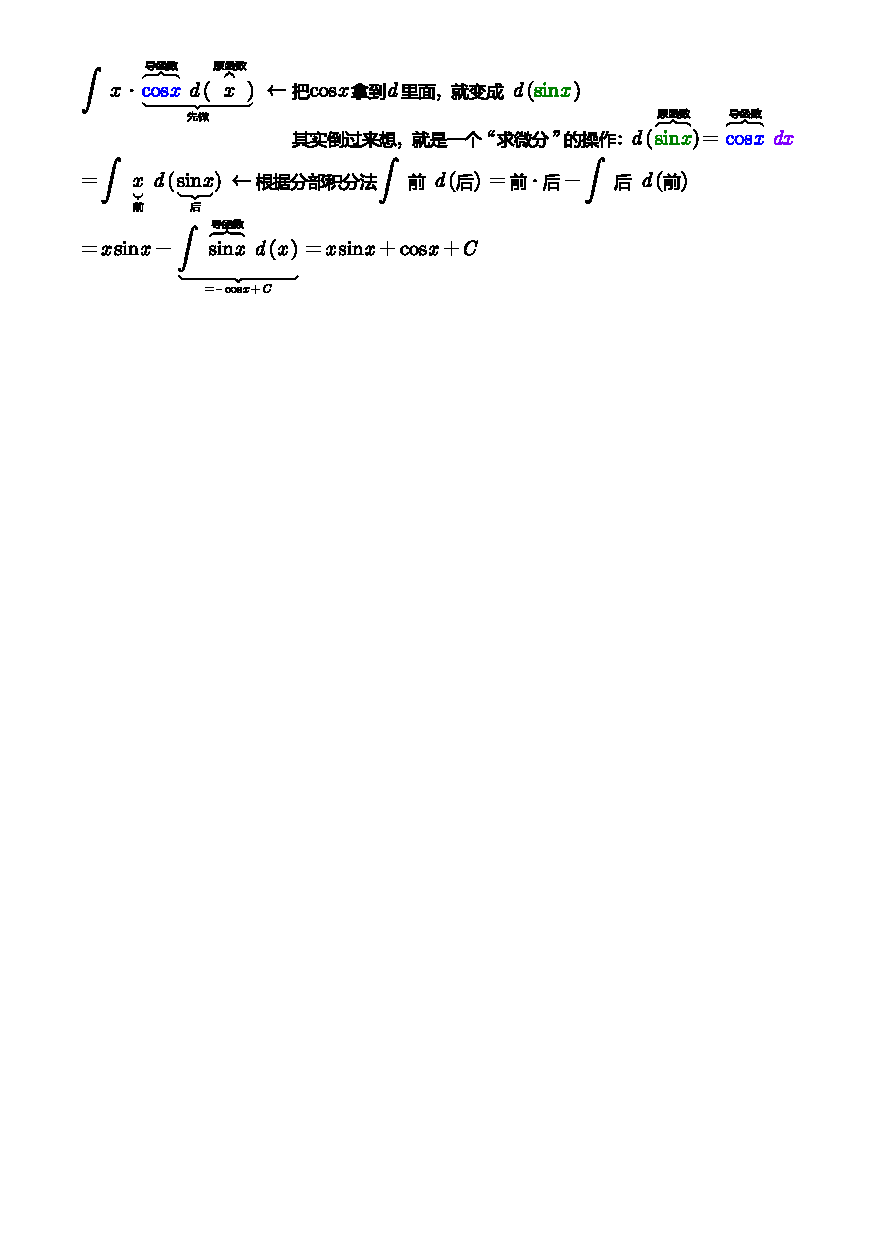
\includegraphics[width=0.95\textwidth]{/0057.pdf}
	\end{myEnvSample}
	
	
	
	
	
	
	
	\section{换元法}
	
	\begin{myEnvSample}
	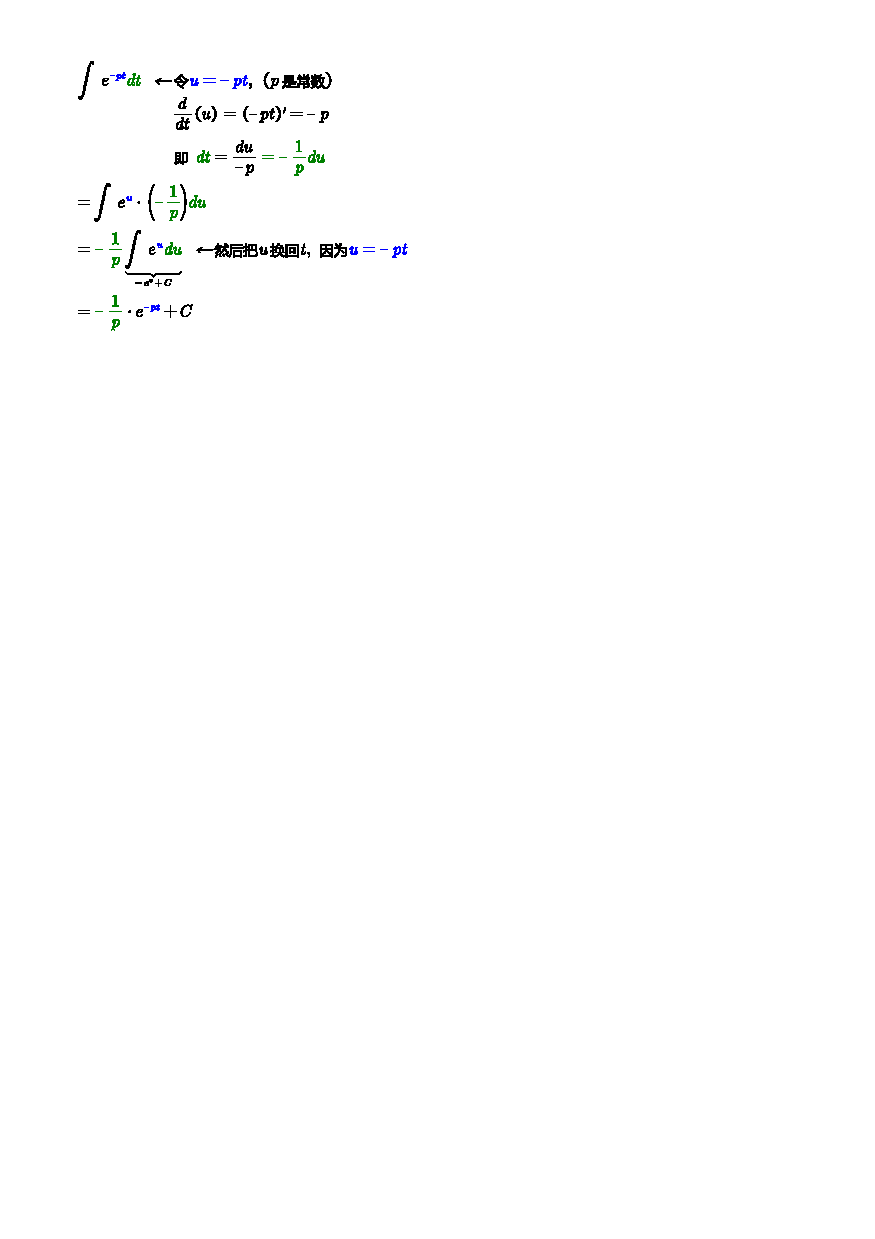
\includegraphics[width=0.5\textwidth]{/0059.pdf}
	\end{myEnvSample}

	上面的换元法, 策略其实就是把一个复杂的数(比如 -pt) 换成(打包成)一个单一的数 (比如u), 然后把原来的dt 也换成用u 表示的du, 先来做u的积分. 做出来后, 再把u 换回(解包)成原来的复杂的数 -pt.
	
	



	
	
	
	
	
	
	
\end{document}


